\section{Scope}
\label{multi-version:scope}

\begin{figure}[t]
  \begin{center}
    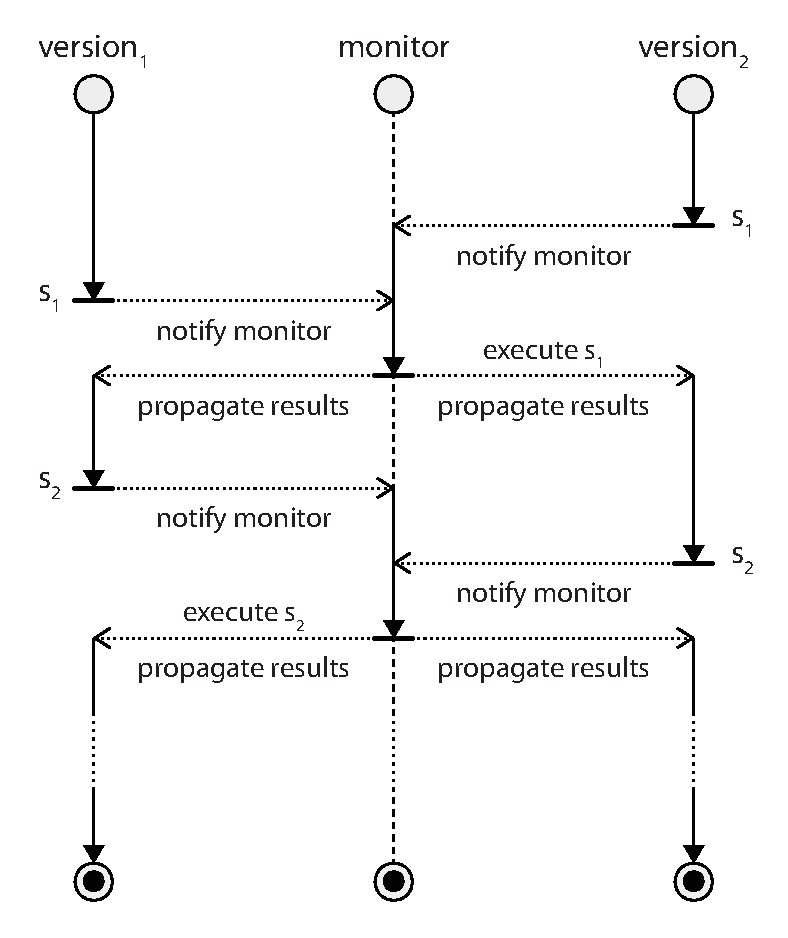
\includegraphics[width=0.5\textwidth]{multi-version/figures/lockstep}
    \caption{Lockstep execution of two version synchronized by the monitor.}
    \label{fig:lockstep-execution}
  \end{center}
\end{figure}

We are restricting our approach to small changes, introduced by software
updates, primarily bug and security fixes. The assumption is that differences
between individual the versions ran in parallel are small. Since our technique
is a runtime technique, we care about differences in behaviour rather than
source code. These are not always correlated, and as shown in
Chapter~\ref{chap:evolution}, the changes to the external behaviour are less
common.

We assume that the sequence of system calls performed by all versions, \ie
their external behaviour, is the same (although various optimizations are
possible as shown in \S\ref{sec:patternmatching}). Given that, we can run all
version in a lockstep as shown in Figure~\ref{fig:lockstep-execution}.  The
monitor runs all versions in parallel. When any of the versions performs a
system call, it notifies the monitor, which then waits for other versions to
perform the system call as well and checks that all versions performed the same
system call by comparing the values of all arguments.

This approach is used by \mx, a prototype system described in
Chapter~\ref{chap:safe-updates}, which implements the failure recovery scheme
and focuses on surviving the crashes caused by bugs introduced by software
updates. To implement this technique, it uses the \ptrace interface.

The lockstep execution allows a precise control over the execution of each
version. The disadvantage is that the application runs at speed of the slowest
version at any given point, which can have a negative impact on the perceived
performance, especially when running large number of versions in parallel. To
address this issue, we can modify this scheme and allow one of the versions,
designated as a leader, to run without waiting for other versions producing a
sequence of system call events, which other versions designated as followers
compare against.

This approach is used by a second system called \varan, described in
Chapter~\ref{chap:efficient-execution}, aimed towards running large number of
versions with low performance overhead, implementing the transparent failover
scheme. To achieve this goal, \varan uses selective binary rewriting.

%%%%%%%%%%%%%%%%%%%%%%

%In this thesis, we present two different designs for building monitors suitable
%for multi-version execution. The first one, called \varan described in
%Chapter~\ref{chap:efficient-execution}, is aimed towards running large number
%of versions side-by-side with low performance overhead, and uses selective
%binary rewriting to achieve this goal. The second one, called \mx , is focused on surviving crashes caused by bugs
%introduced in software updates, with the prototype implementation built using
%the \ptrace mechanism.
